% Instructions: you don't need to change anything in the macros, but
% feel free to define new commands as you wish. Starting from the main
% body, change the specs (e.g., your
% name). use \begin{solution} \end{solution} environment to write your
% solutions. Don't forget to list your collaborators.

\documentclass[12pt,answers]{exam}
%============Macros==================%
\usepackage{amsmath,amsfonts,amssymb,amsthm}
\usepackage[margin=1in]{geometry}
%--------------Cosmetic----------------%
\usepackage{mathtools}
\usepackage{hyperref}
\usepackage{fullpage}
\usepackage{microtype}
\usepackage{xspace}
\usepackage[svgnames]{xcolor}
\usepackage[sc]{mathpazo}
\usepackage{enumitem}
\setlist[enumerate]{itemsep=1pt,topsep=2pt}
\setlist[itemize]{itemsep=1pt,topsep=2pt}
\usepackage{tikz,smartdiagram}
\usetikzlibrary{matrix}
%----------Header--------------------%
\def\course{CS 510/610 Topics on probabilistic graphical models}
\def\term{Portland State U, Winter 2021}
\def\prof{Lecturer: Fang Song}
\newcommand{\handout}[5]{
   \renewcommand{\thepage}{\arabic{page}}
   \begin{center}
   \framebox{
      \vbox{
    \hbox to 5.78in { \hfill \large{\course} \hfill }
       \vspace{2mm}
       \hbox to 5.78in { {\Large \hfill \textbf{#5}  \hfill} }
       \vspace{2mm}
       \hbox to 5.78in { \term \hfill \emph{#2}}
       \hbox to 5.78in { {#3 \hfill \emph{#4}}}
      }
   }
   \end{center}
   \vspace*{4mm}
}
\newcommand{\hw}[4]{\handout{#1}{#2}{#3}{#4}{Homework #1}}

%-----defs and commands-----%
\def\veps{\varepsilon}
\newcommand{\bit}{\{0,1\}}
\newcommand{\negl}{\text{negl}}
\newcommand{\corr}[1]{{\color{blue}{#1}}}
\newcommand{\alg}[1]{\textsf{#1}}
%=======Main document==============%
\begin{document}

%----Specs: change accordingly-----%
\newif\ifstudent % comment out false
 \studenttrue 
% \studentfalse

\def\texbp{5} % bonus for typing in latex
\def\hwnum{1} %
\def\issuedate{01/16/21} % 
\def\duedate{01/28/21} % 
\def\yourname{your name} % type your name here

%------------------------------%
\ifstudent
\hw{\hwnum}{\issuedate}{Student: \yourname}{Due: \duedate}%
\else
\hw{\hwnum}{\issuedate}{\prof}{Due: \duedate}%
\fi

\noindent \textbf{Instructions.} This problem set contains \numpages\
pages (including this cover page) and \numquestions\ questions. A
random subset of problems will be graded.

\begin{itemize}
\item Your solutions will be graded on \emph{correctness} and
  \emph{clarity}. You should only submit work that you believe to be
  correct, and you will get significantly more partial credit if you
  clearly identify the gap(s) in your solution. It is good practice to
  start any long solution with an informal (but accurate) summary that
  describes the main idea. You may opt for the ``I take 15\%'' option.

\item You need to submit a PDF file before the deadline. Either a
  clear scan of you handwriting or a typeset document is accepted. You
  will get $\texbp$ bonus points for typing in LaTeX (Download and use
  the accompany TeX file).

\item You may collaborate with others on this problem set.  However,
  you must \textbf{{write up your own solutions}} and \textbf{{list
      your collaborators and any external sources}} for each
  problem. Be ready to explain your solutions orally to a course staff
  if asked.

\end{itemize}

\newpage

\begin{questions}

  \question (Probability)
  \begin{parts}
    \part[5] Let $A,B,C$ be random variables, and suppose that the
    joint distribution is positive. Prove or disprove the following
    statement. If $A\perp B |C$ and $A\perp C |B$, then $A\perp B$ and
    $A\perp C$. 
    
    \part[10] Let $X$ be a set of random variables with joint distribution
    $p$. Let $A,B,C$ be three disjoint subsets of variables such that
    $X = A\cup B \cup C$. Prove that $A \perp B | C$ \textbf{iff.} we
    can write $p$ in the form $p(X) = \phi_1(A,\corr{C}) \phi_2(B,C)$ for
    some non-negative functions $\phi_1$ and $\phi_2$. 
    \part[10] Let $X,Y,Z$ be random variables. Show that
    $p(X|Y) = \sum_z p(X,z|Y)$. (Hint: chain rule) 
  \end{parts}
  
  % \begin{solution}
  %  uncomment the environment and write your solution here
  % \end{solution}

  \newpage 
  \question[10] (Detecting cycle in a graph) Describe an algorithm to
  determine if a given directed graph $G$ contains a cycle. Show
  correctness and running time of your algorithm.


  \newpage

  \question (Bayesian networks) For each of the following statements,
  state True or False, and briefly justify your answers.

  \begin{parts}
    \part[6] Let $\mathcal{G}$ be the BN shown in Fig.~\ref{fig:bn1}.

    \begin{figure}[h!]
      \centering
      \begin{tikzpicture}
        \matrix (m) [matrix of math nodes,row sep=2em,column
        sep=3em,minimum width=2em] { A & B & C \\
          D & E & \\};

        \path[-stealth]

        (m-1-1) edge (m-1-2)
        
        (m-1-2) edge (m-1-3)

        (m-2-1) edge (m-2-2)

        (m-2-1) edge (m-1-2)
        
        ; 
          \end{tikzpicture}

      \caption{A Bayesian network}
      \label{fig:bn1}      
    \end{figure}
    \begin{enumerate}[label=(\arabic*)]
    \item $E \perp C | B$.
    \item $A \perp E | C$. 
    \end{enumerate}
    \newpage 
    \part[9] Read the diagram in Fig.~\ref{fig:rel}. Recall the
    definitions of local and global independencies of a BN
    $\mathcal{G}$ and independencies of a distribution $p$.
    \begin{align*}
      I_\ell(\mathcal{G}) = &\{ X\perp \text{NonDescendants}(X) |
                              \text{Pa}(X) \} \\
      I(\mathcal{G}) = &\{ X\perp Y |Z : \text{d-Sep}(X,Y|Z)\} \\
      I(p) = &\{ X\perp Y |Z : p(X,Y|Z) = p(X|Z) p(Y|Z)\}
    \end{align*}
    
    \begin{figure}[h!]
      \centering
      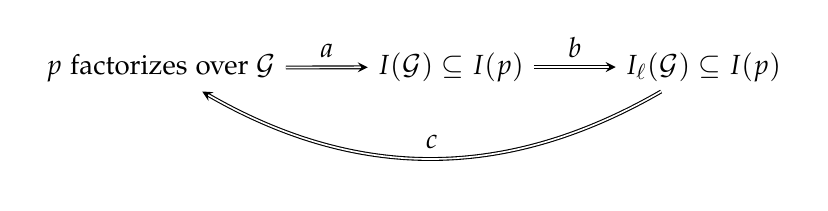
\begin{tikzpicture}
        \matrix (m) [matrix of math nodes,row sep=3em,column
        sep=3em,minimum width=2em] {
          p \text{ factorizes over } \mathcal{G} & I(\mathcal{G})
          \subseteq I(p) & I_\ell (\mathcal{G}) \subseteq I(p)\\};

        \path[-stealth]
        (m-1-1) edge [double] node [above]
        {$a$} (m-1-2)
        
        (m-1-2) edge [double] node [above] {$b$} (m-1-3)

        (m-1-3) edge [bend left, double] node [above] {$c$} (m-1-1)
        ; 
          \end{tikzpicture}
      \caption{Some relations in Bayesian networks.}
      \label{fig:rel}
    \end{figure}

    \begin{enumerate}[label=(\arabic*)]
    \item Relation $a$ is true. 
    \item Relation $b$ is true.
    \item Relation $c$ is true.
    \end{enumerate}
    \newpage
    \part[5] If $\mathcal{G}_1$ is an $I$-map of distribution $p$, and
    $\mathcal{G}_1$ has fewer edges than $\mathcal{G}_2$, then
    $\mathcal{G}_2$ is not a minimal $I$-map of $p$.
  \end{parts}

\end{questions}


\end{document}

